\chapter{System Integration and Testing}

How did everything go together? As a whole the drone, cameras, processing and mapping all have a specific process, and if followed, one can come to a reasonable result. To replicate the project, it will require a setup phase to build a drone, test each component, and to calibrate the cameras. The active phase will consist of image acquisition, and processing which can be done in the cloud. \\

One of the issues encountered upon was when attempting to fly a mission as in Figure \ref{fig:longridge_waypoints}. The GPS and compass didn't work. It is most likely caused by interference induced by the high current draw, and would require shielding to prevent against it from happening. The solution may be non-trivial, as it may require electromagnetic simulations and design to solve the problem.

\begin{figure}[H]
\centering
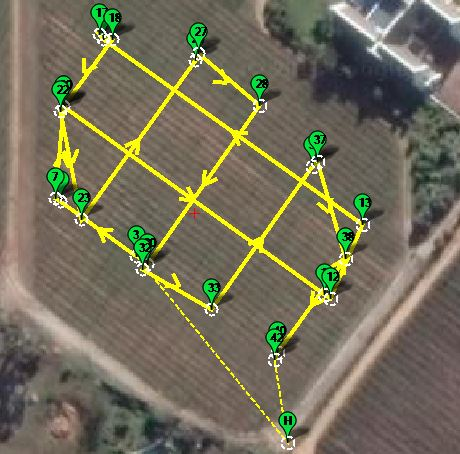
\includegraphics[scale=0.4]{images/longridge_waypoints.jpg}
\caption{Mission waypoints at Longridge}
\label{fig:longridge_waypoints}
\end{figure}

%quick discussion, issues
%
%testing, + results, + analysis
%
%Capabilities, works well, could be better, compared to this solution. Parrot Sequoia. Quite affordable. Complexity?

\section{Parrot Sequia}

The Parrot Sequoia, as mentioned in Section \ref{sec:lit}, costs \$3500. It has 5 cameras. A 16 MP RGB camera, and 4 1.2 MP cameras capturing green, red, red-edge and NIR bands of light.

\begin{figure}[H]
\begin{subfigure}{0.5\textwidth}
\centering
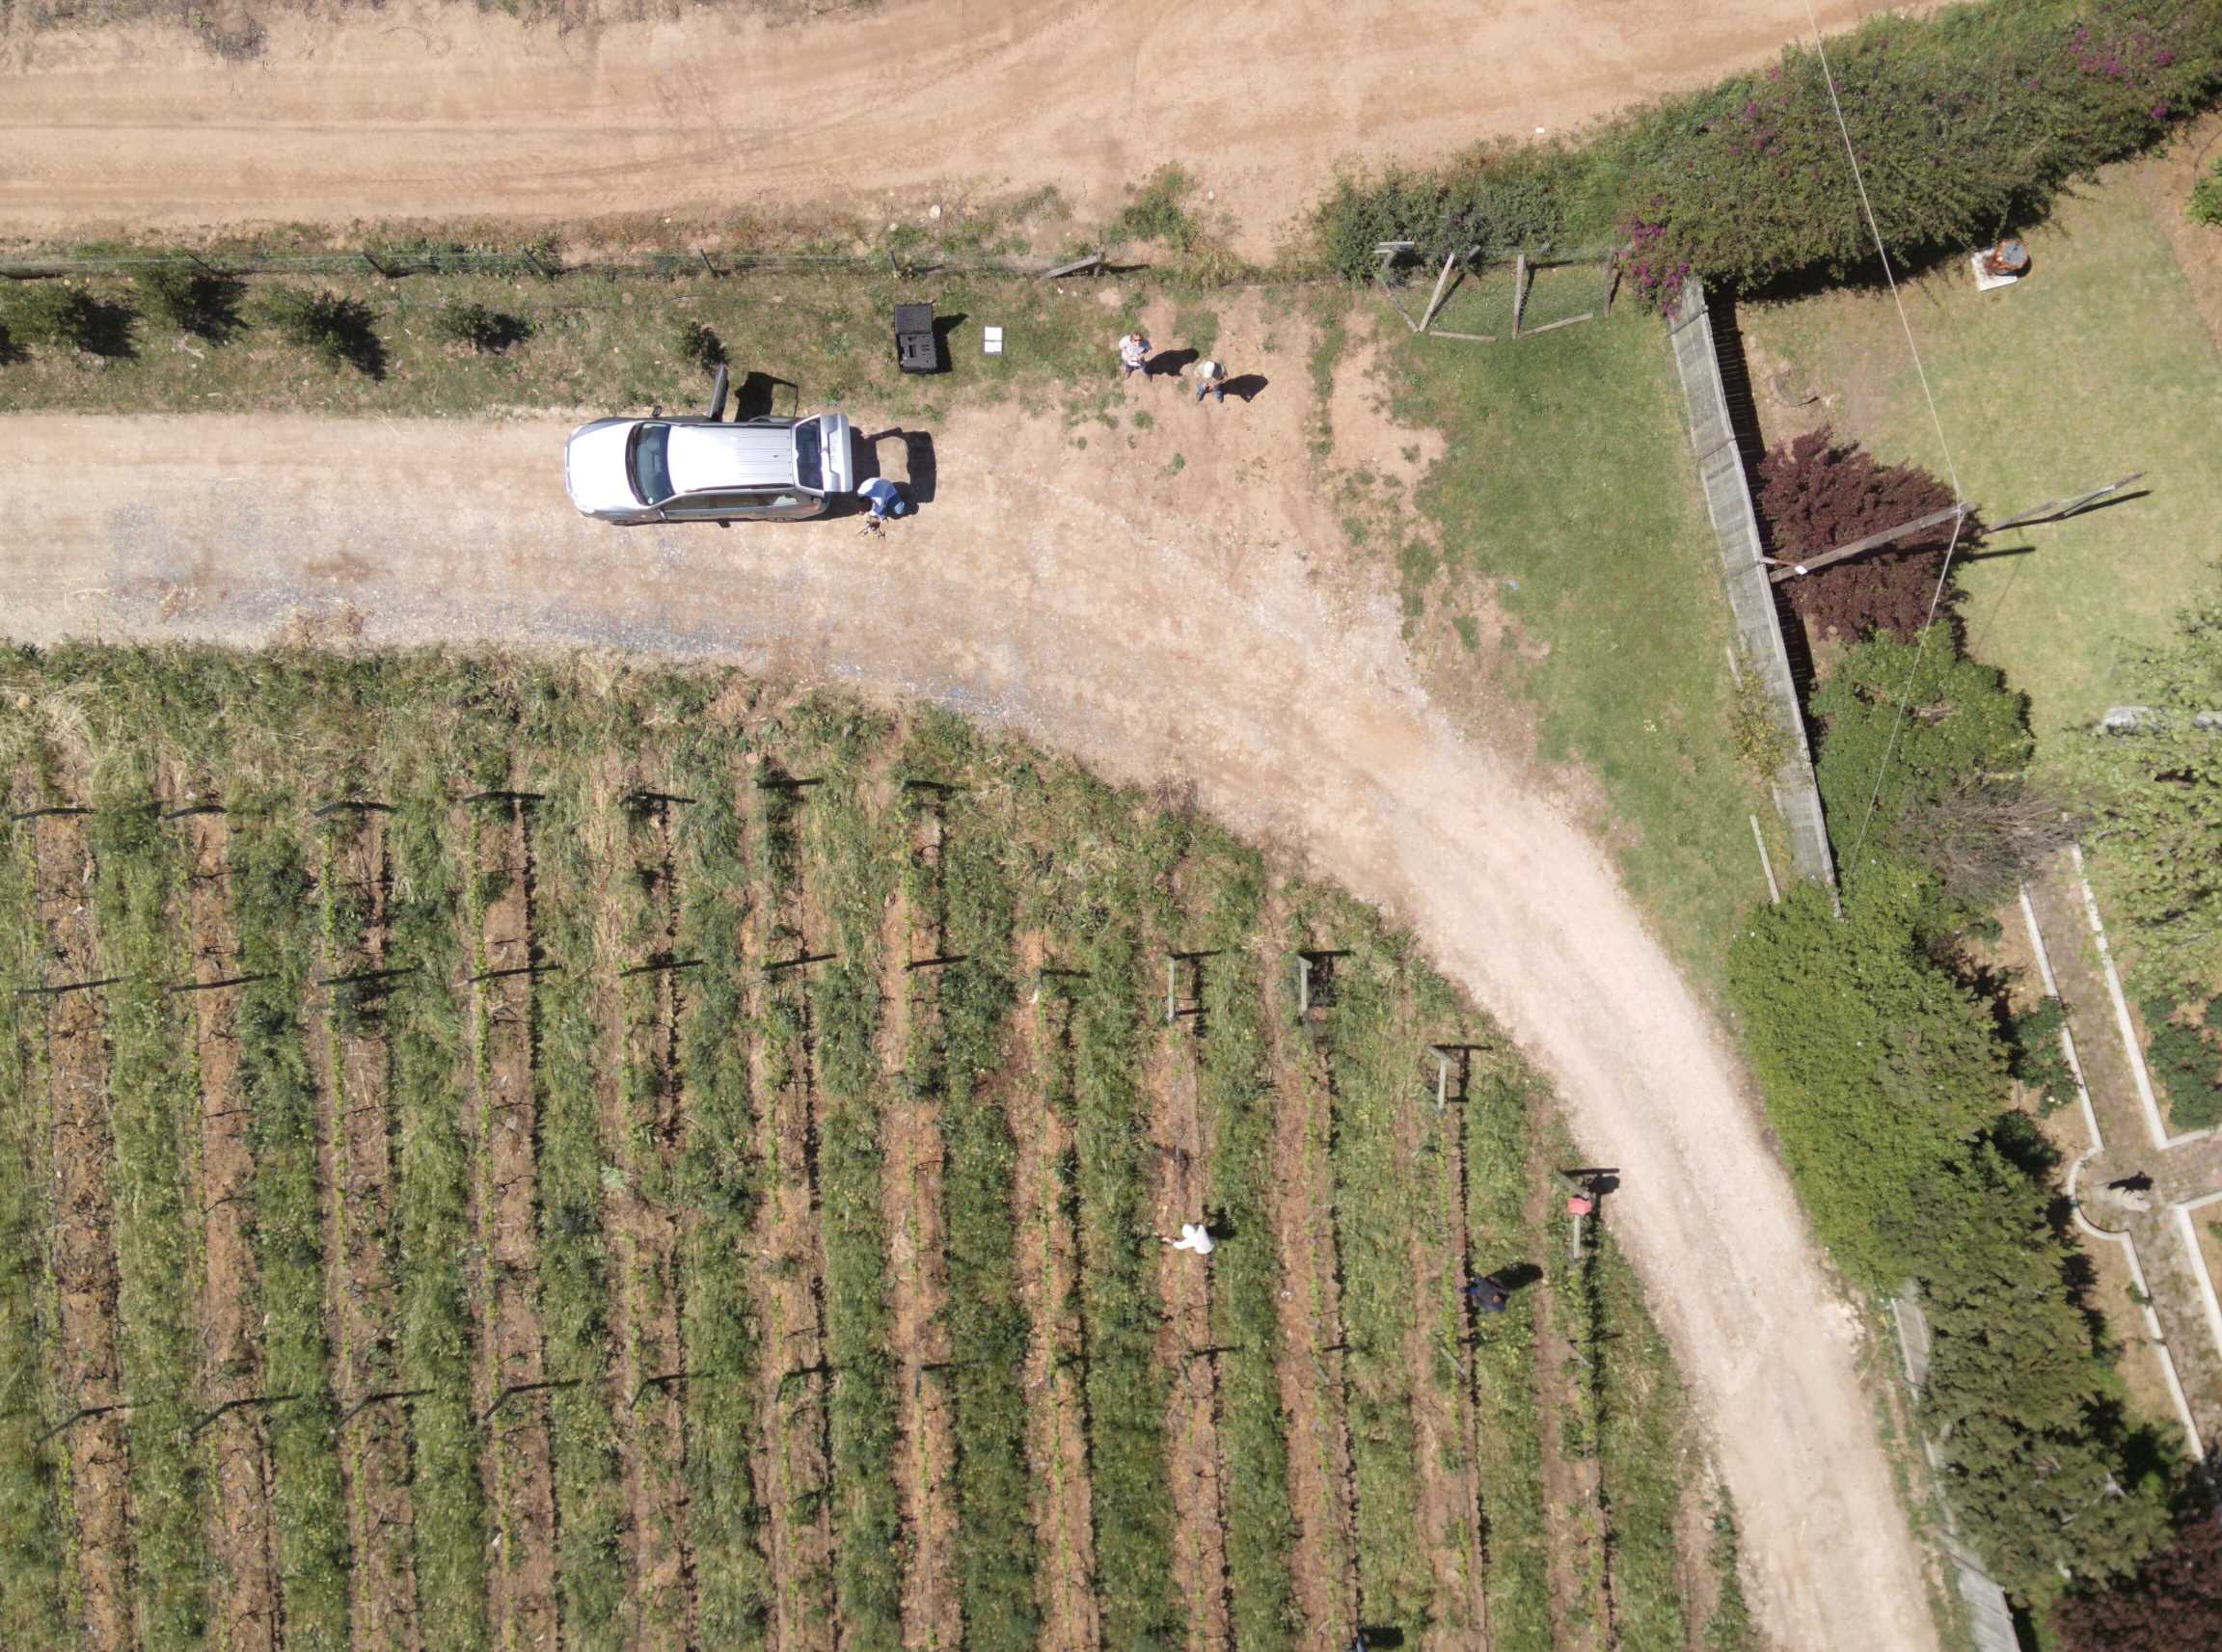
\includegraphics[scale=0.11]{images/sequoia_rgb.jpg}
\caption{Sequoia RGB image}
\end{subfigure}
\begin{subfigure}{0.5\textwidth}
\centering
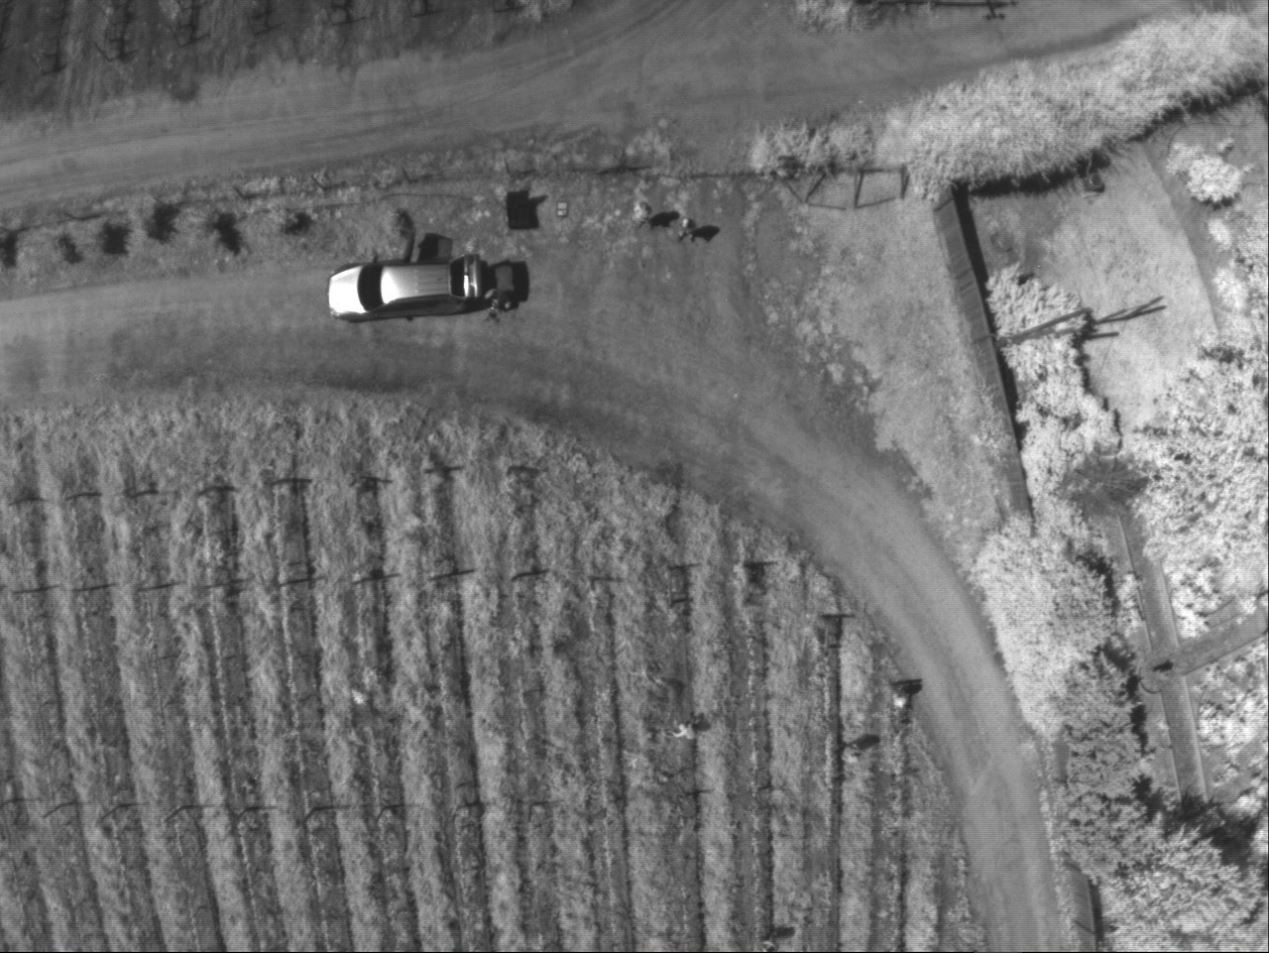
\includegraphics[scale=0.2]{images/sequoia_nir.jpg}
\caption{Sequoia NIR image}
\end{subfigure}
\caption{Parrot Sequoia images}
\label{fig:sequoia}
\end{figure}

\begin{figure}[H]
\centering
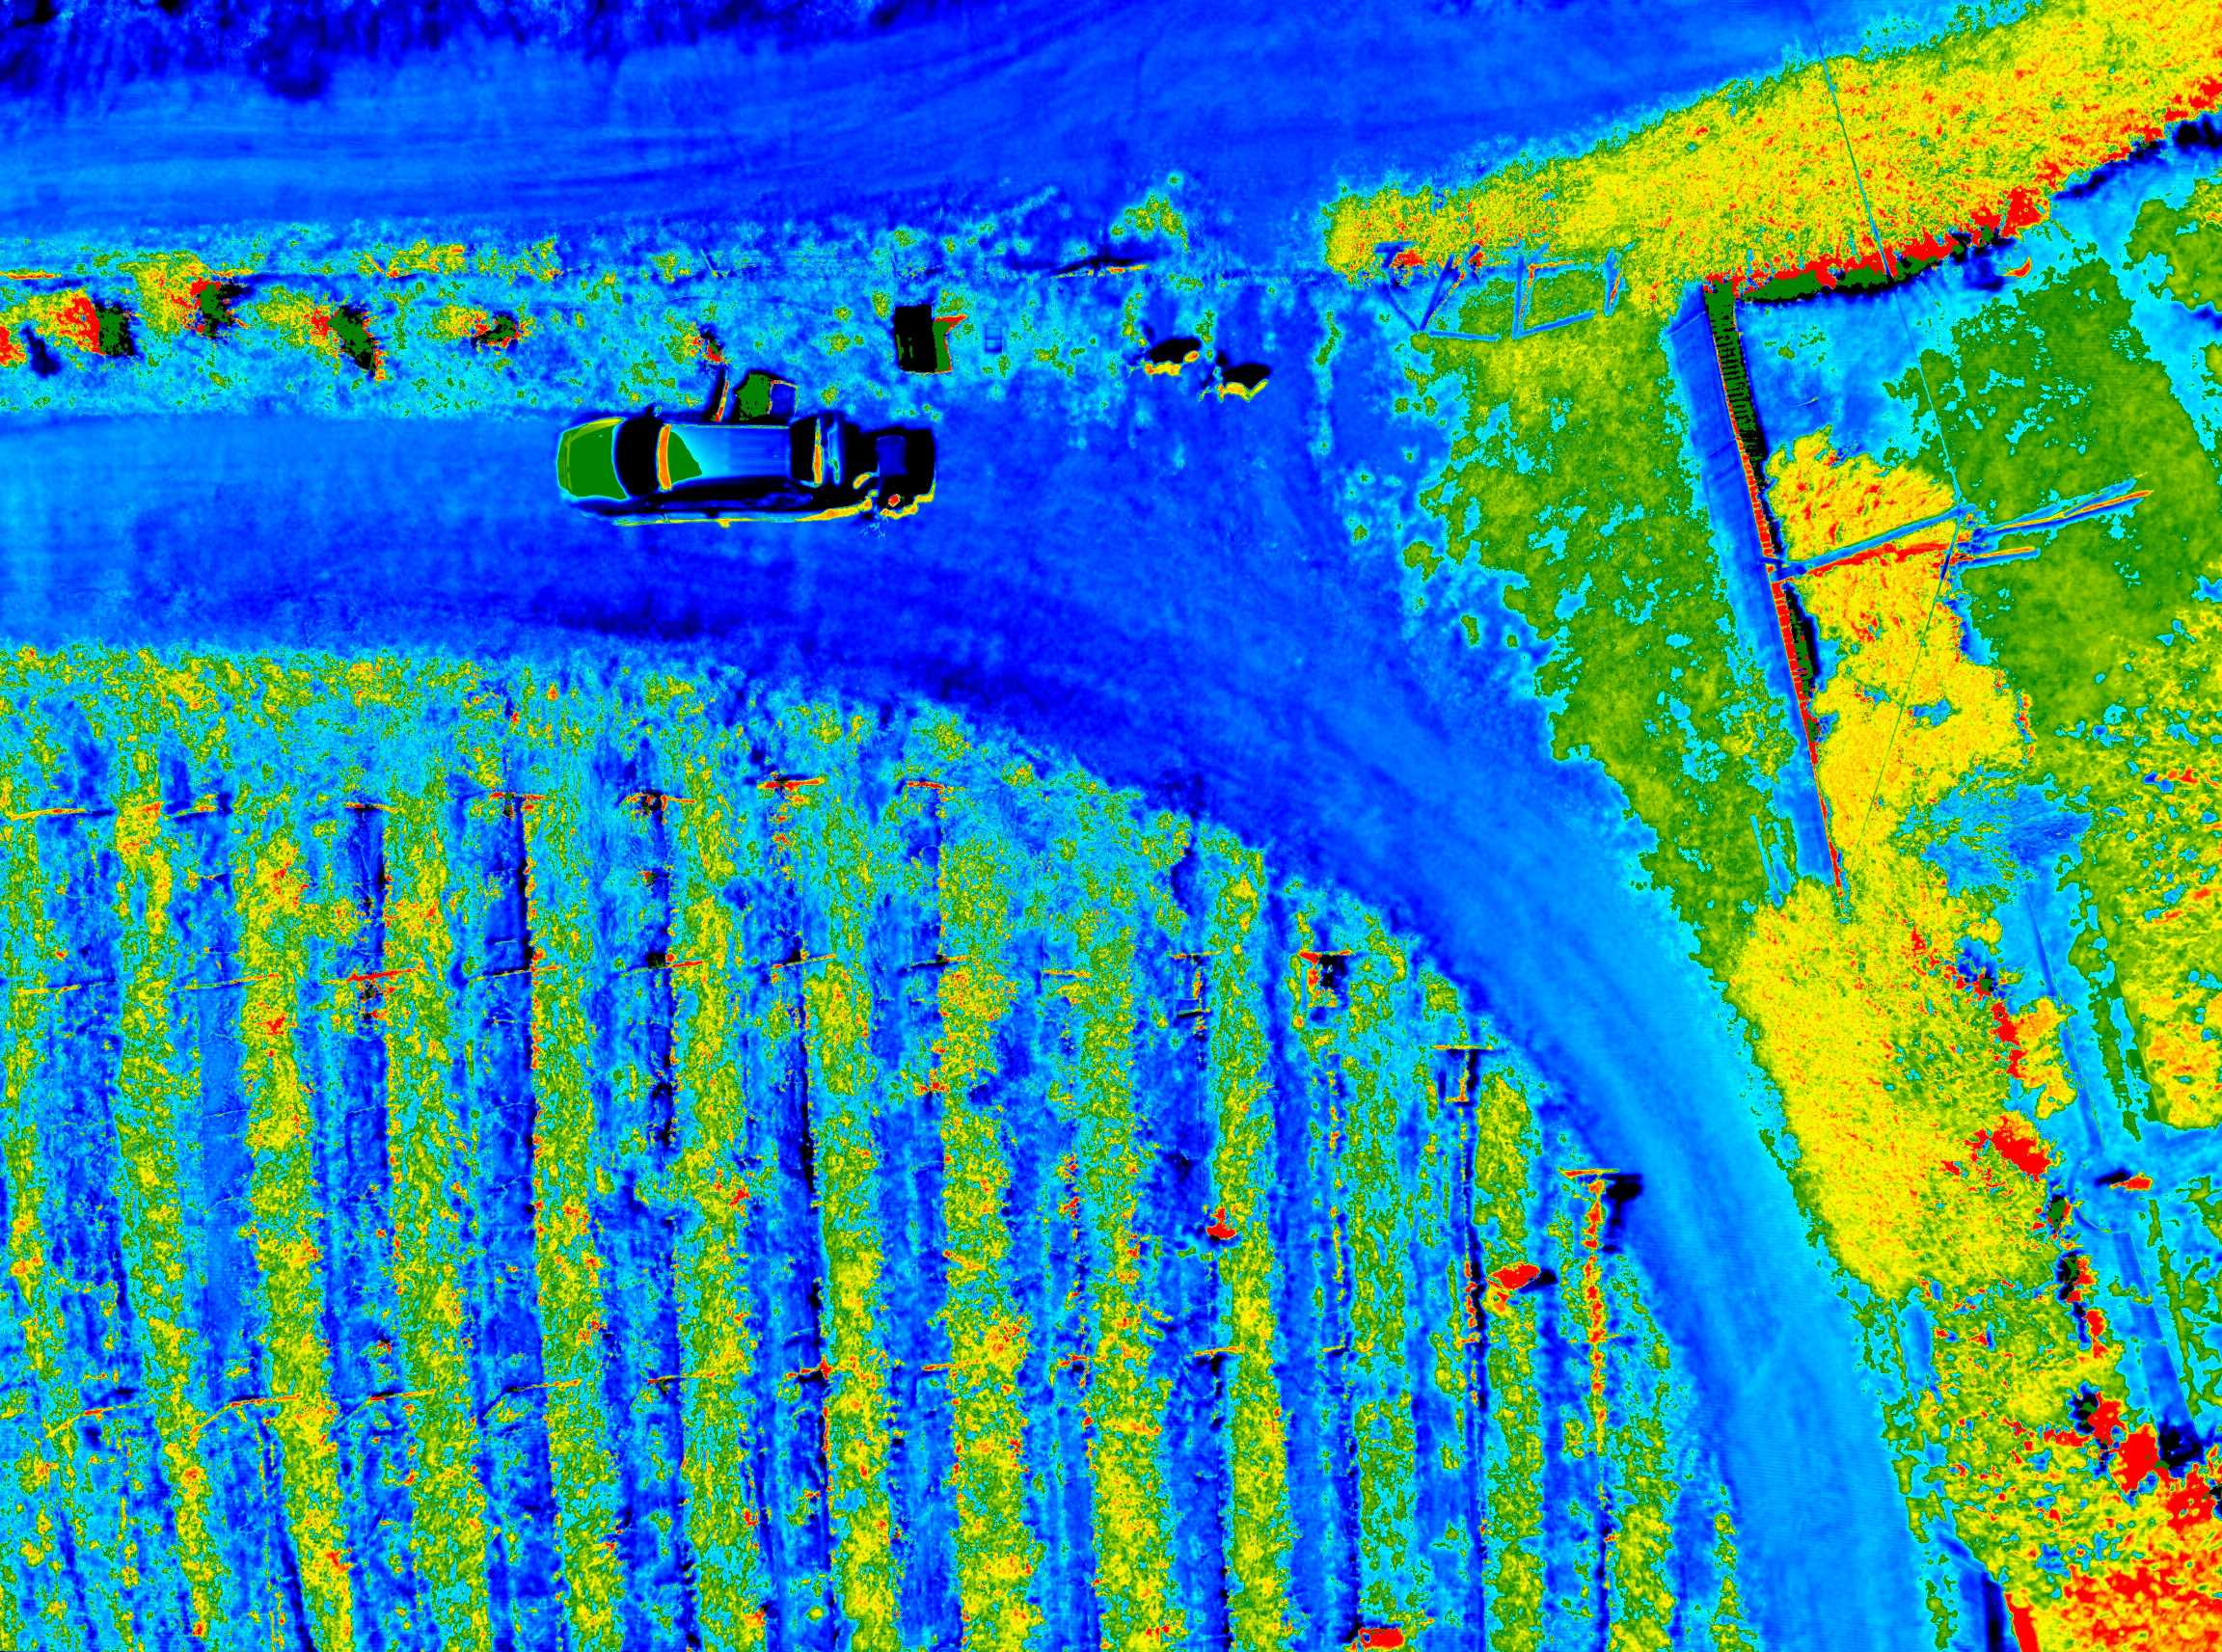
\includegraphics[scale=0.11]{images/sequoia_ndvi.jpg}
\caption{Resulting NDVI of images as in Figure \ref{fig:sequoia}}
\label{fig:sequoia_ndvi}
\end{figure}

NDVI values for the grass in-between the vines range between 0.22 and 0.27. The vines them-self were still too young, and could not be discerned from the picture.

\begin{figure}[H]
\centering
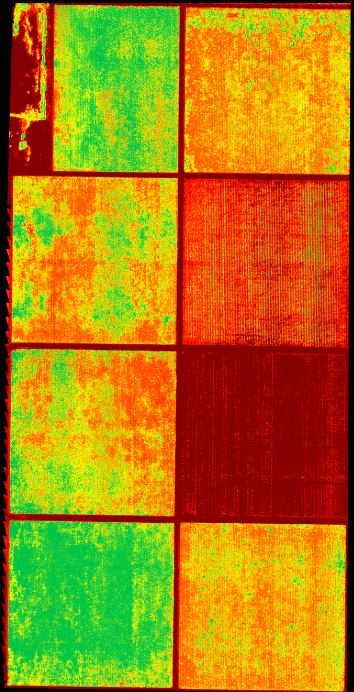
\includegraphics[scale=0.3]{images/chris_example_ndvi.JPG}
\caption{Typical NDVI using Sequoia for grapes by Chris}
\label{fig:chris_ndvi}
\end{figure}

The NDVI is relative and depends on the plant in question and also the density of what has been surveyed. It is a function of both the red absorbtion and NIR reflection. Also, the NDVI value will change depending on lighting conditions and the exact parts of the spectrum that the sensor picks up. For healthy dense canopy grapes as in the bottom left of Figure \ref{fig:chris_ndvi} an NDVI value over 0.65 or 0.7 is pretty good for the Sequoia sensor. The actual reflection in the specific band varies a great deal for healthy plants in different lighting and that’s why a normalised index is used. Chris, \cite{chris}.\\

The setup used in this project seems promising, and needs further investigation and testing for refinement. In future, it may be possible to build a self-charging system, completely autonomous, and cost-effective for every farmer.